
\documentclass[tikz]{standalone}
\usepackage{graphicx}
\usepackage{amsmath, amssymb, amsfonts}
\usetikzlibrary{calc}
\newcommand{\R}{\mathcal{R}}

\begin{document}

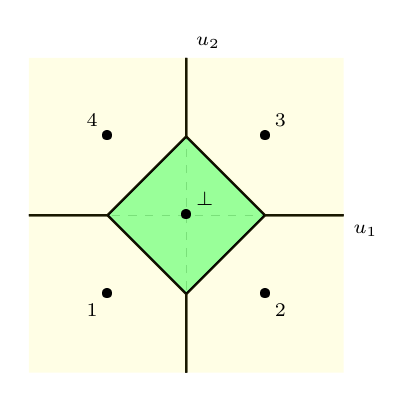
\begin{tikzpicture}
\draw[dashed, opacity=0.2] (-2,0) -- (2,0) node[anchor=north west, opacity=1]{\scriptsize $u_1$};
\draw[dashed, opacity=0.2] (0,-2) -- (0,2)node[anchor=south west, opacity=1]{\scriptsize $u_2$};

\draw[thick, fill=green, opacity = 0.4] (1,0) -- (0,1) -- (-1,0) -- (0,-1) -- cycle;
\draw[thick] (2,0) -- (1,0) -- (0,1) -- (0,2);
\draw[thick] (0,2) -- (0,1) -- (-1,0) -- (-2,0);
\draw[thick] (-2,0) -- (-1,0) -- (0,-1) -- (0,-2);
\draw[thick] (0,-2) -- (0,-1) -- (1,0) -- (2,0);

\path[fill=yellow, opacity = 0.1] (2,0) -- (1,0) -- (0,1) -- (0,2) -- (2,2) -- cycle;
\path[fill=yellow, opacity = 0.1] (0,2) -- (0,1) -- (-1,0) -- (-2,0) -- (-2, 2)-- cycle;
\path[fill=yellow, opacity = 0.1] (-2,0) -- (-1,0) -- (0,-1) -- (0,-2) -- (-2,-2) -- cycle;
\path[fill=yellow, opacity = 0.1] (0,-2) -- (0,-1) -- (1,0) -- (2,0) -- (2,-2) -- cycle;

\node at (-1,-1){\textbullet} (-1,-1)node[anchor=north east]{\scriptsize $1$};
\node at (1,-1){\textbullet} (1,-1)node[anchor= north west]{\scriptsize $2$};
\node at (1,1){\textbullet} (1,1)node[anchor= south west]{\scriptsize $3$};
\node at (-1,1){\textbullet} (-1,1)node[anchor=south east]{\scriptsize $4$};
\node at (0,0){\textbullet} node[anchor=south west]{\scriptsize $\bot$};
\end{tikzpicture}


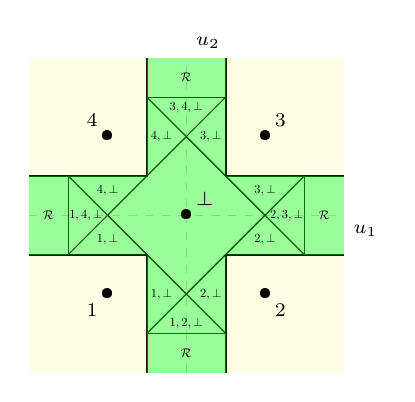
\begin{tikzpicture}
\draw[dashed, opacity=0.2] (-2,0) -- (2,0) node[anchor=north west, opacity=1]{\scriptsize $u_1$};
\draw[dashed, opacity=0.2] (0,-2) -- (0,2)node[anchor=south west, opacity=1]{\scriptsize $u_2$};

%boxes around each outcome region
\draw[thick] (1/2, 2) -- (1/2, 1/2) -- (2, 1/2);
\draw[thick] (2,-1/2) -- (1/2, -1/2) -- (1/2, -2);
\draw[thick] (-2, 1/2) -- (-1/2, 1/2) -- (-1/2, 2);
\draw[thick] (-2, -1/2) -- (-1/2, -1/2) -- (-1/2, -2);



%lines for subsets
\draw (-3/2, -1/2) -- (1/2, 3/2);
\draw (3/2, -1/2) -- (-1/2, 3/2);
\draw (-1/2, -3/2) -- (3/2, 1/2);
\draw (-3/2, 1/2) -- (1/2, -3/2);

\draw (3/2, -1/2) -- (3/2, 1/2);
\draw (-3/2, -1/2) -- (-3/2, 1/2);
\draw (-1/2, 3/2) -- (1/2, 3/2);
\draw (-1/2, -3/2) -- (1/2, -3/2);

%outcome cell shading
\path[fill=yellow, opacity = 0.1] (2,1/2) -- (1/2,1/2) -- (1/2,2) -- (2,2) -- cycle;
\path[fill=yellow, opacity = 0.1] (-1/2,2) -- (-1/2,1/2) -- (-2,1/2) -- (-2,2) -- cycle;
\path[fill=yellow, opacity = 0.1] (-2,-1/2) -- (-1/2,-1/2) -- (-1/2,-2) -- (-2,-2) -- cycle;
\path[fill=yellow, opacity = 0.1] (1/2,-2) -- (1/2,-1/2) -- (2,-1/2) -- (2,-2) -- cycle;

\draw[fill=green, opacity = 0.4] (1,0) -- (0,1) -- (-1,0) -- (0,-1) -- cycle;

%mark regions where we map to any report
\path[fill=green, opacity=0.4] (-2, 1/2) -- (-3/2, 1/2) -- (-3/2, -1/2) -- (-2, -1/2) -- cycle;
\path[fill=green, opacity=0.4] (2, 1/2) -- (3/2, 1/2) -- (3/2, -1/2) -- (2, -1/2) -- cycle;
\path[fill=green, opacity=0.4] (-1/2, -2) -- (-1/2, -3/2) -- (1/2, -3/2) -- (1/2, -2) -- cycle;
\path[fill=green, opacity=0.4] (-1/2, 2) -- (-1/2, 3/2) -- (1/2, 3/2) -- (1/2, 2) -- cycle;

%where you have two optimal reports
\path[fill=green, opacity=0.4] (-3/2, -1/2) -- (-1,0) -- (-1/2, -1/2) -- cycle;
\path[fill=green, opacity=0.4] (-1/2, -3/2) -- (0,-1) -- (-1/2, -1/2) -- cycle;
\path[fill=green, opacity=0.4] (3/2, -1/2) -- (1,0) -- (1/2, -1/2) -- cycle;
\path[fill=green, opacity=0.4] (1/2, -3/2) -- (0,-1) -- (1/2, -1/2) -- cycle;
\path[fill=green, opacity=0.4] (1/2, 3/2) -- (0,1) -- (1/2, 1/2) -- cycle;
\path[fill=green, opacity=0.4] (3/2, 1/2) -- (1,0) -- (1/2, 1/2) -- cycle;
\path[fill=green, opacity=0.4] (-3/2, 1/2) -- (-1,0) -- (-1/2, 1/2) -- cycle;
\path[fill=green, opacity=0.4] (-1/2, 3/2) -- (0,1) -- (-1/2, 1/2) -- cycle;

%three optimal reports
\path[fill=green, opacity=0.4] (-1/2, -3/2) -- (0,-1) -- (1/2, -3/2) -- cycle;
\path[fill=green, opacity=0.4] (-3/2, -1/2) -- (-1,0) -- (-3/2, 1/2) -- cycle;
\path[fill=green, opacity=0.4] (3/2, -1/2) -- (1,0) -- (3/2, 1/2) -- cycle;
\path[fill=green, opacity=0.4] (-1/2, 3/2) -- (0,1) -- (1/2, 3/2) -- cycle;

%all the labels
\node at (-1,-1){\textbullet} (-1,-1)node[anchor=north east]{\scriptsize $1$};
\node at (1,-1){\textbullet} (1,-1)node[anchor= north west]{\scriptsize $2$};
\node at (1,1){\textbullet} (1,1)node[anchor= south west]{\scriptsize $3$};
\node at (-1,1){\textbullet} (-1,1)node[anchor=south east]{\scriptsize $4$};
\node at (0,0){\textbullet} node[anchor=south west]{\scriptsize$\bot$};
\node at (-7/4, 0){\scalebox{0.45}{$\R$}};
\node at (7/4, 0){\scalebox{0.45}{$\R$}};
\node at (0, -7/4){\scalebox{0.45}{$\R$}};
\node at (0, 7/4){\scalebox{0.45}{$\R$}};
\node at (-1, -5/16){\scalebox{0.45}{$1,\bot$}};
\node at (-5/16, -1){\scalebox{0.45}{$1,\bot$}};
\node at (1, -5/16){\scalebox{0.45}{$2,\bot$}};
\node at (5/16, -1){\scalebox{0.45}{$2,\bot$}};
\node at (5/16, 1){\scalebox{0.45}{$3,\bot$}};
\node at (1, 5/16){\scalebox{0.45}{$3,\bot$}};
\node at (-1, 5/16){\scalebox{0.45}{$4,\bot$}};
\node at (-5/16, 1){\scalebox{0.45}{$4,\bot$}};
\node at (0, -11/8){\scalebox{0.45}{$1,2,\bot$}};
\node at (-5.1/4,0){\scalebox{0.45}{$1,4,\bot$}};
\node at (5.1/4,0){\scalebox{0.45}{$2,3,\bot$}};
\node at (0, 11/8){\scalebox{0.45}{$3,4,\bot$}};

\end{tikzpicture}
% % % % % % % % % % % % % % % % % % % % % % % % % % % %
%l1 regions
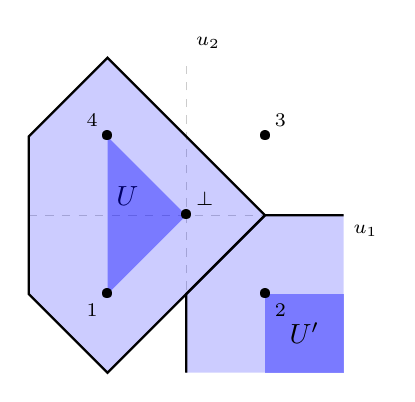
\begin{tikzpicture}
\draw[dashed, opacity=0.2] (-2,0) -- (2,0) node[anchor=north west, opacity=1]{\scriptsize $u_1$};
\draw[dashed, opacity=0.2] (0,-2) -- (0,2)node[anchor=south west, opacity=1]{\scriptsize $u_2$};

%U_{1,4,\bot}
\draw[thick,fill=blue, fill opacity=0.2] (-2,-1) -- (-2,1) -- (-1,2) -- (1, 0) -- (-1,-2) -- cycle;
\node at (-3/4,1/4){$U$};
\path[fill=blue, opacity=0.4] (-1,1) -- (0,0) -- (-1,-1) --cycle;

%U_{2}
\path[fill=blue, opacity=0.2] (0,-2) -- (0,-1) -- (1,0) -- (2,0) -- (2,-2) -- cycle;
\path[fill=blue, fill opacity=0.4] (1,-1) -- (2,-1) -- (2,-2) -- (1, -2) -- cycle;
\node at (3/2,-3/2){$U'$};
\draw[thick] (0,-2) -- (0,-1) -- (1,0) -- (2,0);


\node at (-1,-1){\textbullet} (-1,-1)node[anchor=north east]{\scriptsize $1$};
\node at (1,-1){\textbullet} (1,-1)node[anchor= north west]{\scriptsize $2$};
\node at (1,1){\textbullet} (1,1)node[anchor= south west]{\scriptsize $3$};
\node at (-1,1){\textbullet} (-1,1)node[anchor=south east]{\scriptsize $4$};
\node at (0,0){\textbullet} node[anchor=south west]{\scriptsize $\bot$};

\end{tikzpicture}
% % % % % % % % % % % % % % % % % % % % % % % % % % % % %
%l infinity regions
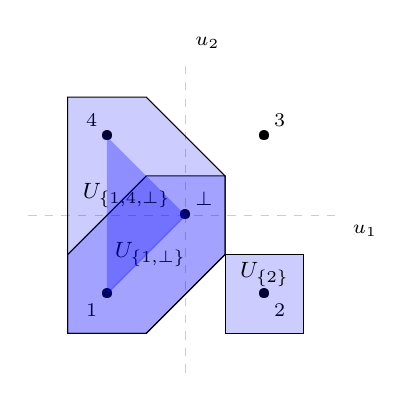
\begin{tikzpicture}
%background
\draw[dashed, opacity=0.2] (-2,0) -- (2,0) node[anchor=north west, opacity=1]{\scriptsize $u_1$};
\draw[dashed, opacity=0.2] (0,-2) -- (0,2)node[anchor=south west, opacity=1]{\scriptsize $u_2$};

\node at (-1,-1){\textbullet} (-1,-1)node[anchor=north east]{\scriptsize $1$};
\node at (1,-1){\textbullet} (1,-1)node[anchor= north west]{\scriptsize $2$};
\node at (1,1){\textbullet} (1,1)node[anchor= south west]{\scriptsize $3$};
\node at (-1,1){\textbullet} (-1,1)node[anchor=south east]{\scriptsize $4$};
\node at (0,0){\textbullet} node[anchor=south west]{\scriptsize $\bot$};

%region for U_{1,\bot}
\draw[fill=blue, fill opacity=0.2] (-3/2,-3/2) -- (-3/2,-1/2) -- (-1/2,1/2) -- (1/2, 1/2) -- (1/2, -1/2) -- (-1/2, -3/2) -- cycle;
\node at (-0.45,-1/2){\footnotesize $U_{\{1,\bot\}}$};
\draw[blue, opacity=0.3] (0,0) -- (-1,-1) --cycle;

%region for U_{2}
\draw[fill=blue, fill opacity=0.2] (3/2,-3/2) -- (3/2,-1/2) -- (1/2,-1/2) -- (1/2, -3/2) -- cycle;
\node at (1,-3/4){\footnotesize $U_{\{2\}}$};

%region for U_{1,4,\bot}
\draw[fill=blue, fill opacity=0.2] (-3/2,-3/2) -- (-3/2,3/2) -- (-1/2,3/2) -- (1/2, 1/2) -- (1/2, -1/2) -- (-1/2, -3/2) -- cycle;
\node at (-3/4, 1/4){\footnotesize $U_{\{1,4,\bot\}}$};
\path[fill=blue, opacity=0.3] (-1,1) -- (0,0) -- (-1,-1) --cycle;

\end{tikzpicture}


\end{document}
%%% Local Variables:
%%% mode: latex
%%% TeX-master: t
%%% End:
